\documentclass[11pt]{article}

\usepackage[utf8]{inputenc}
\usepackage[margin=1in]{geometry} 
\usepackage{amsmath,amsthm,amssymb,graphicx,mathtools,tikz,hyperref,multicol,cancel,enumitem,booktabs,float,pgfplots,multirow,mathrsfs,textcomp,gensymb,soul,changepage,threeparttable}
%\usepackage[table]{xcolor}
\usepackage[T1]{fontenc}
\usepackage[italian]{babel}
\usepackage{hyphenat}
\hyphenation{mate-mati-ca recu-perare}
\usetikzlibrary{positioning}
\pgfplotsset{compat=1.14}

\newcommand{\n}{\mathbb{N}}
\newcommand{\z}{\mathbb{Z}}
\newcommand{\q}{\mathbb{Q}}
\newcommand{\cx}{\mathbb{C}}
\newcommand{\real}{\mathbb{R}}
\newcommand{\field}{\mathbb{F}}
\newcommand{\ita}[1]{\textit{#1}}
\newcommand{\com}[2]{#1\backslash#2}
\newcommand{\oneton}{\{1,2,3,...,n\}}
\newcommand{\idea}[1]{\begin{gather*}#1\end{gather*}}
\newcommand{\ef}{\ita{f} }
\newcommand{\eff}{\ita{f}}
\newcommand{\proofs}[1]{\begin{proof}#1\end{proof}}
\newcommand{\inv}[1]{#1^{-1}}
\newcommand{\setb}[1]{\{#1\}}
\newcommand{\en}{\ita{n }}
\newcommand{\vbrack}[1]{\langle #1\rangle}
\newcommand{\qRa}{\quad \Rightarrow \quad}
\newcommand{\smaca}[1]{\textbf{\textsc{#1}}}

\newenvironment{theorem}[2][Teorema]{\begin{trivlist}
\item[\hskip \labelsep {\bfseries #1}\hskip \labelsep {\bfseries #2.}]}{\end{trivlist}}
\newenvironment{lemma}[2][Lemma]{\begin{trivlist}
\item[\hskip \labelsep {\bfseries #1}\hskip \labelsep {\bfseries #2.}]}{\end{trivlist}}
\newenvironment{exercise}[2][Esercizio]{\begin{trivlist}
\item[\hskip \labelsep {\bfseries #1}\hskip \labelsep {\bfseries #2.}]}{\end{trivlist}}
\newenvironment{proposition}[2][Proposizione]{\begin{trivlist}
\item[\hskip \labelsep {\bfseries #1}\hskip \labelsep {\bfseries #2.}]}{\end{trivlist}}
\newenvironment{corollary}[2][Corollario]{\begin{trivlist}
\item[\hskip \labelsep {\bfseries #1}\hskip \labelsep {\bfseries #2.}]}{\end{trivlist}}

\hypersetup {
    colorlinks,
    linkcolor=blue
}

\graphicspath{{img/}}

\begin{document}
\setlength{\parindent}{0pt}
\title{\vspace{-4em}{\large Laboratorio di Meccanica e Termodinamica} \\
    Relazione di Laboratorio}
\author{GRUPPO 3\\
        Gerardo Selce, Emanuela Galluccio}
\date{10/12/2024}
\maketitle

\vspace{-2em}\par\noindent\rule{\textwidth}{0.4pt}
\begin{center}
    {\Large\sc Misura del coefficiente di attrito statico}
\end{center}
\par\noindent\rule{\textwidth}{0.4pt}

\section{Introduzione}

Scopo dell'esperienza è la determinazione del coefficiente di attrito statico di due superfici di un blocchetto di legno. Dopo aver agganciato il blocchetto ad una molla (con coefficiente di elasticità $k$ noto) è stato misurato il suo allungamento minimo tale da mettere in movimento il blocchetto, per quindici volte. Questo esperimento è stato iterato per otto masse diverse posizionate sul blocchetto di legno, per entrambe le superfici prese in considerazione. Dalla seconda legge della dinamica otteniamo l'espressione
\begin{equation}
    k\Delta l=\mu_smg
\end{equation}
Che descrive la relazione tra forza elastica e forza di attrito statico, dalla quale si ricaverà il coefficiente di attrito statico $\mu_s$.

\section{Richiami teorici}

Il coefficiente di attrito statico è un parametro che descrive la forza di attrito tra due superfici a riposo relativo. É indicato con il simbolo $\mu_s$ è rappresenta il rapporto tra la massima forza di attrito statico e la forza normale esercitata tra le due superfici. Questa grandezza è priva di unità di misura perchè rappresenta un rapporto tra due forze.
\begin{equation}
    \mu_s = \frac{F_{attrito statico}}{F_{normale}}
\end{equation}
in cui
\begin{itemize}
    \item $F_{attritostatico}$ è la massima forza di attrito che può agire senza che avvenga movimento.
    \item $F_{normale}$ è la forza normale, ovvero la componente della forza perpendicolare alla superficie di contatto.
\end{itemize}
Il valore $\mu_s$ dipende dalla natura delle superfici (materiale, rugosità, presenza di lubrificanti, ecc).

\subsection{Richiami Matematici}
Il metodo dei minimi quadrati è una tecnica che permette di trovare una funzione, rappresentata da una curva di regressione, che si avvicini il più possibile ad un insieme di dati (tipicamente punti del piano). In particolare, la funzione trovata deve essere quella che minimizza la somma dei quadrati delle distanze tra i dati osservati e quelli della curva che rappresenta la funzione stessa. Siano $b$ il coefficiente angolare e $a$ l'intercetta della retta di regressione:
\begin{equation}
    b=\frac{\displaystyle\sum_{i=1}^{N}[(x_i-\overline{x})(y_i-\overline{y})]}{\displaystyle\sum_{i=1}^{N}(x_i-\overline{x})^2}
\end{equation}
\begin{equation}
    a=\overline{y}-b\overline{x}
\end{equation}
Con $\overline{x}=\frac{\displaystyle\sum_{i=1}^{N}x_i}{N}$ e $\overline{y}=\frac{\displaystyle\sum_{i=1}^{N}y_i}{N}$
mentre le incertezze:
\begin{equation}
    \Delta b=3\sigma_b
\end{equation}
\begin{equation}
    \Delta a=3\sigma_a
\end{equation}
Con $$\sigma_b=\sigma_y\sqrt{\frac{N}{\Delta}}$$
$$\sigma_y=\sqrt{\frac{\displaystyle\sum_{i=1}^{N}(y_i-bx_i-a)^2}{N-2}}$$
$$\sigma_a=\sigma_y\sqrt{\frac{\displaystyle\sum_{i=1}^{N}x_i^2}{\Delta}}$$
$$\Delta=N\displaystyle\sum_{i=1}^{N}(x_i-\overline{x})^2$$

\section{Apparato sperimentale}

Per svolgere quest'esperienza è stato utilizzato il seguente apparato sperimentale:
\begin{itemize}
    \item Riga millimetrica
    \item Molla in acciaio
    \item Rondelle metalliche
    \item Bilancia digitale
    \item Blocchetto in legno
\end{itemize}

\begin{table}[H]
\centering
\begin{tabular}{|c|c|}
\hline
\textbf{Strumenti di misura} & \textbf{Risoluzione} \\
\hline
Riga millimetrica & $1\ mm$ \\
Bilancia digitale & $0.01\ g$ \\
\hline
\end{tabular}
\caption{Risoluzione degli strumenti di misura utilizzati}
\label{tab:}
\end{table}

\begin{figure}[H]
  \centering
  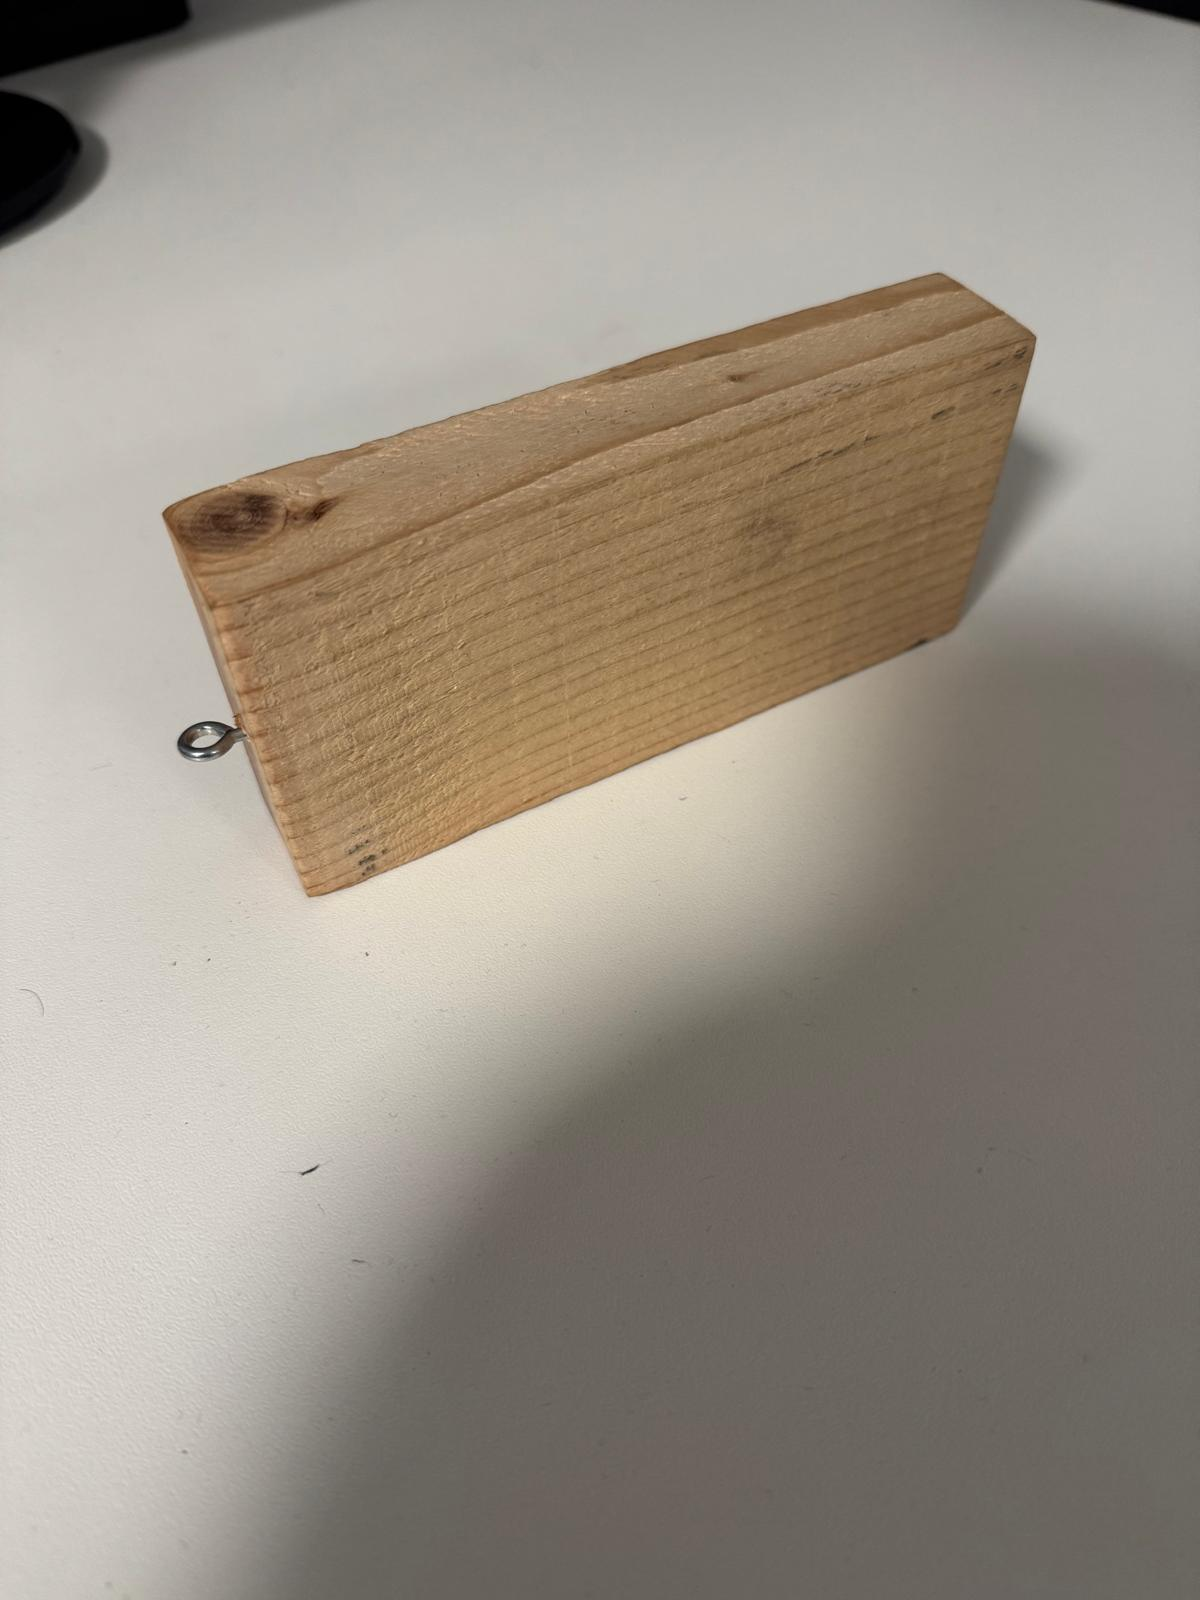
\includegraphics[width=0.55\textwidth]{legno.jpg}
  \caption{Blocchetto di legno utilizzato per l'esperimento. La prima superficie presa in considerazione è quella su cui poggia in figura. La seconda è quella più estesa rivolta verso la fotocamera.}
\end{figure}
\begin{figure}[H]
  \centering
  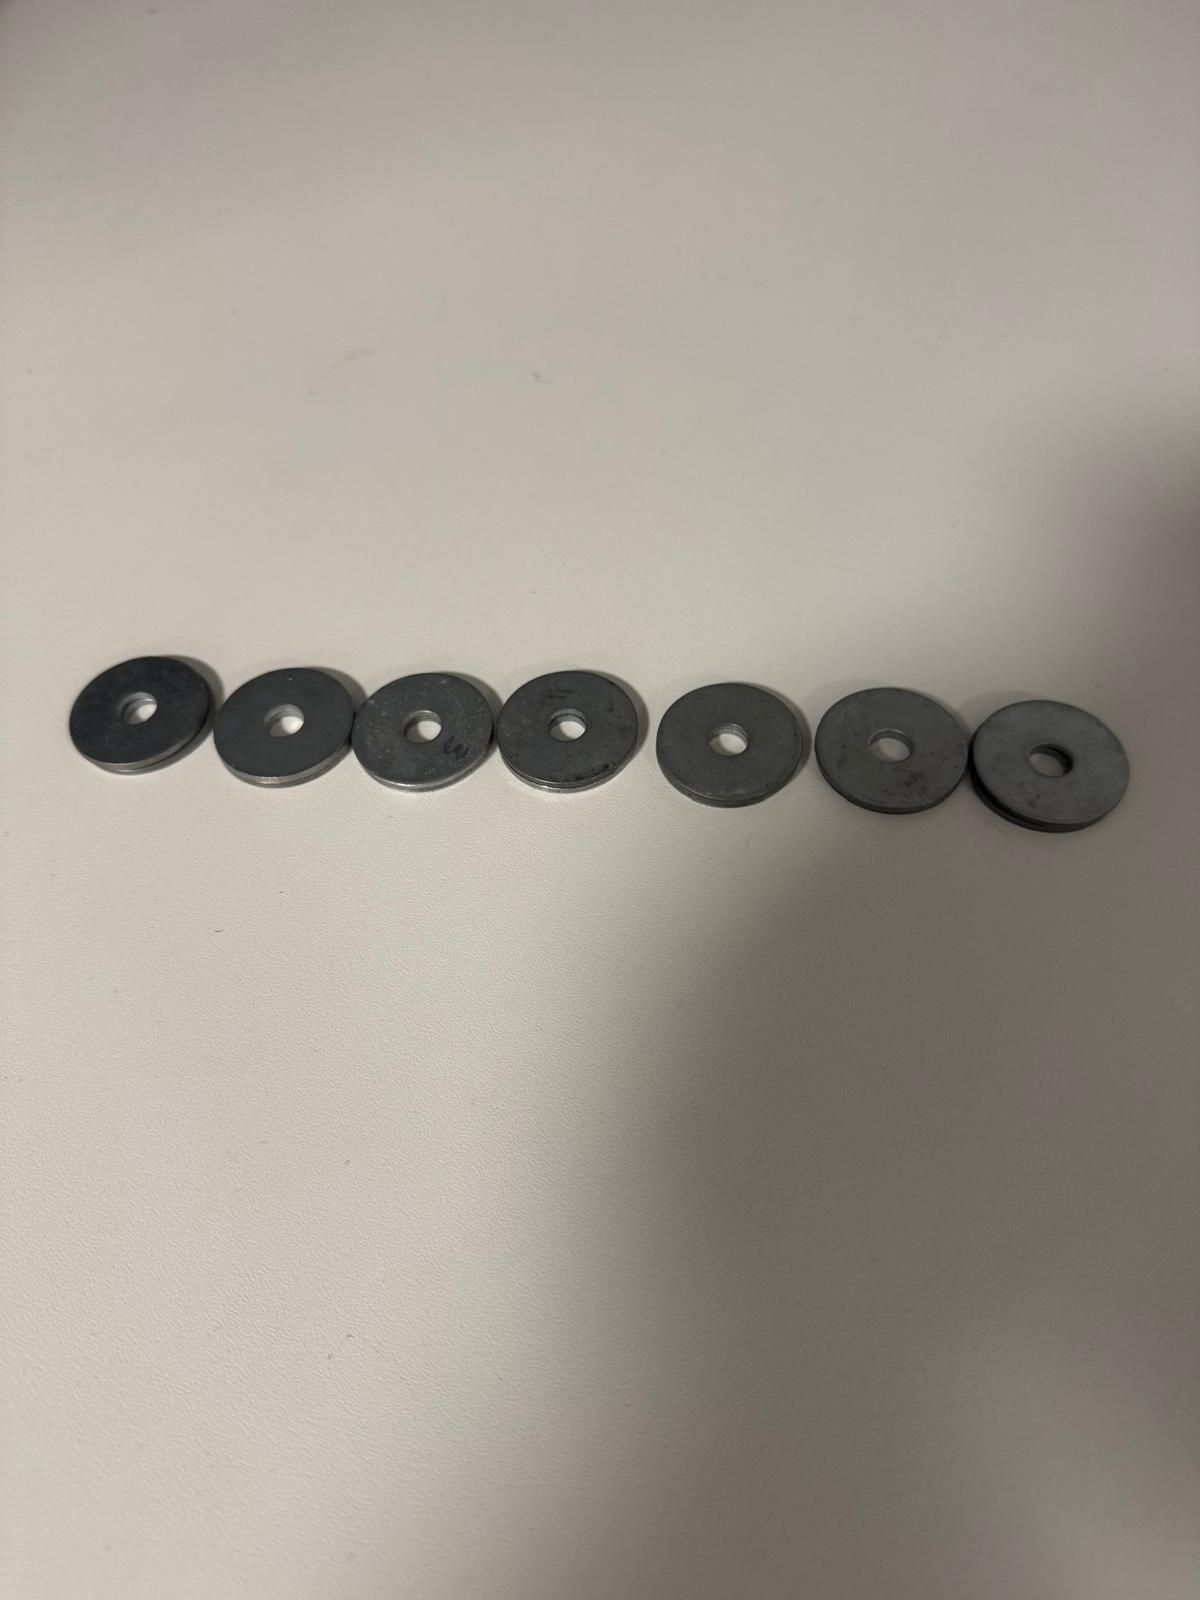
\includegraphics[width=0.55\textwidth]{rondelle.jpg}
  \caption{Rondelle utilizzate per l'esperimento. Sono raggruppate in coppie per un totale di sette gruppi. L'ottava massa considerata per l'esperimento è il blocchetto di legno scarico di rondelle.}
\end{figure}

\section{Descrizione e analisi dei dati sperimentali}

Abbiamo innanzitutto stabilito le otto masse da agganciare alla molla. Il valore di ognuna è stato ottenuto calcolando la media di tre diverse misurazioni ottenute con la bilancia digitale e la loro incertezza è pari a quella strumentale (la semidispersione dei risultati è minore dell'errore strumentale).

\begin{table}[H]
\centering
\begin{tabular}{|c|}
\hline
\textbf{$m_i$ ($g$)}\\
\hline
$121.69\pm 0.01$ \\
$144.16\pm 0.01$ \\
$166.67\pm 0.01$ \\
$189.00\pm 0.01$ \\
$210.69\pm 0.01$ \\
$233.21\pm 0.01$ \\
$255.74\pm 0.01$ \\
$277.94\pm 0.01$ \\
\hline
\end{tabular}
\caption{La tabella mostra le otto masse utilizzate per l'esperimento. L'aumento segue un andamento pressocchè lineare poichè le coppie di rondelle aggiunte hanno quasi la stessa massa.}
\label{tab:}
\end{table}
Per ognuna delle masse considerate sono state effettuate quindici misurazioni di allungamento della molla. Il valore finale è stato stimato come punto medio tra la misura più piccola e più grande ottenute, mentre l’incertezza sulla misura è stata valutata con la semidispersione, poichè il suo valore risulta maggiore della risoluzione strumentale. Conoscendo la costante elastica della molla ($k=3\ \frac{N}{m}$) è possibile calcolare, dalla Legge (1), il modulo della forza elastica per ogni $\Delta l$ e, per ogni massa $m$, calcolare il modulo della forza normale.

\subsection{Prima superficie}

\subsubsection{Prima massa}
\begin{table}[H]
\centering
\begin{tabular}{|c|c|}
\hline
\textbf{N°} & \textbf{$\Delta l_1$ ($cm$)}\\
\hline
$1$ & $13.00\pm 0.05$ \\
\hline
$2$ & $13.00\pm 0.05$ \\
\hline
$3$ & $12.00\pm 0.05$ \\
\hline
$4$ & $11.00\pm 0.05$ \\
\hline
$5$ & $10.50\pm 0.05$ \\
\hline
$6$ & $14.00\pm 0.05$ \\
\hline
$7$ & $11.00\pm 0.05$ \\
\hline
$8$ & $10.00\pm 0.05$ \\
\hline
$9$ & $11.00\pm 0.05$ \\
\hline
$10$ & $11.00\pm 0.05$ \\
\hline
$11$ & $13.00\pm 0.05$ \\
\hline
$12$ & $10.70\pm 0.05$ \\
\hline
$13$ & $11.00\pm 0.05$ \\
\hline
$14$ & $10.80\pm 0.05$ \\
\hline
$15$ & $11.00\pm 0.05$ \\
\hline
\end{tabular}
\caption{Allungamenti misurati per la prima massa.}
\label{tab:}
\end{table}
L'allungamento della molla è quindi:
\begin{equation}
    \Delta l_1=(12.00\pm 2.00)\ cm
\end{equation}
La forza elastica generata dalla molla è uguale a:
\begin{equation}
    F_{elastica_1} = (0.36\pm 0.06)\ N
\end{equation}
La forza normale agente sul blocchetto di legno è uguale a:
\begin{equation}
    F_{N_1} = (1.1938\pm 0.0001)\ N
\end{equation}

\subsubsection{Seconda massa}
\begin{table}[H]
\centering
\begin{tabular}{|c|c|}
\hline
\textbf{N°} & \textbf{$\Delta l_2$ ($cm$)}\\
\hline
$1$ & $11.50\pm 0.05$ \\
\hline
$2$ & $11.50\pm 0.05$ \\
\hline
$3$ & $15.50\pm 0.05$ \\
\hline
$4$ & $11.50\pm 0.05$ \\
\hline
$5$ & $15.50\pm 0.05$ \\
\hline
$6$ & $14.50\pm 0.05$ \\
\hline
$7$ & $14.00\pm 0.05$ \\
\hline
$8$ & $11.50\pm 0.05$ \\
\hline
$9$ & $13.50\pm 0.05$ \\
\hline
$10$ & $13.50\pm 0.05$ \\
\hline
$11$ & $12.00\pm 0.05$ \\
\hline
$12$ & $11.00\pm 0.05$ \\
\hline
$13$ & $11.00\pm 0.05$ \\
\hline
$14$ & $15.00\pm 0.05$ \\
\hline
$15$ & $15.00\pm 0.05$ \\
\hline
\end{tabular}
\caption{Allungamenti misurati per la seconda massa.}
\label{tab:}
\end{table}
L'allungamento della molla è quindi:
\begin{equation}
    \Delta l_2=(13.25\pm 2.25)\ cm
\end{equation}
La forza elastica generata dalla molla è uguale a:
\begin{equation}
    F_{elastica_2} = (0.40\pm 0.07)\ N
\end{equation}
La forza normale agente sul blocchetto di legno è uguale a:
\begin{equation}
    F_{N_2} = (1.4142\pm 0.0001)\ N
\end{equation}


\subsubsection{Terza massa}
\begin{table}[H]
\centering
\begin{tabular}{|c|c|}
\hline
\textbf{N°} & \textbf{$\Delta l_3$ ($cm$)}\\
\hline
$1$ & $12.00\pm 0.05$ \\
\hline
$2$ & $12.50\pm 0.05$ \\
\hline
$3$ & $14.50\pm 0.05$ \\
\hline
$4$ & $15.00\pm 0.05$ \\
\hline
$5$ & $14.50\pm 0.05$ \\
\hline
$6$ & $13.50\pm 0.05$ \\
\hline
$7$ & $12.00\pm 0.05$ \\
\hline
$8$ & $13.00\pm 0.05$ \\
\hline
$9$ & $13.80\pm 0.05$ \\
\hline
$10$ & $15.00\pm 0.05$ \\
\hline
$11$ & $13.00\pm 0.05$ \\
\hline
$12$ & $13.50\pm 0.05$ \\
\hline
$13$ & $14.00\pm 0.05$ \\
\hline
$14$ & $15.00\pm 0.05$ \\
\hline
$15$ & $13.50\pm 0.05$ \\
\hline
\end{tabular}
\caption{Allungamenti misurati per la terza massa.}
\label{tab:}
\end{table}
L'allungamento della molla è quindi:
\begin{equation}
    \Delta l_3=(13.50\pm 1.50)\ cm
\end{equation}
La forza elastica generata dalla molla è uguale a:
\begin{equation}
    F_{elastica_3} = (0.41\pm 0.05)\ N
\end{equation}
La forza normale agente sul blocchetto di legno è uguale a:
\begin{equation}
    F_{N_3} = (1.6350\pm 0.0001)\ N
\end{equation}

\subsubsection{Quarta massa}
\begin{table}[H]
\centering
\begin{tabular}{|c|c|}
\hline
\textbf{N°} & \textbf{$\Delta l_4$ ($cm$)}\\
\hline
$1$ & $16.00\pm 0.05$ \\
\hline
$2$ & $17.00\pm 0.05$ \\
\hline
$3$ & $17.00\pm 0.05$ \\
\hline
$4$ & $15.00\pm 0.05$ \\
\hline
$5$ & $18.00\pm 0.05$ \\
\hline
$6$ & $15.00\pm 0.05$ \\
\hline
$7$ & $18.50\pm 0.05$ \\
\hline
$8$ & $15.50\pm 0.05$ \\
\hline
$9$ & $18.00\pm 0.05$ \\
\hline
$10$ & $17.50\pm 0.05$ \\
\hline
$11$ & $14.50\pm 0.05$ \\
\hline
$12$ & $16.00\pm 0.05$ \\
\hline
$13$ & $16.00\pm 0.05$ \\
\hline
$14$ & $15.00\pm 0.05$ \\
\hline
$15$ & $15.00\pm 0.05$ \\
\hline
\end{tabular}
\caption{Allungamenti misurati per la quarta massa.}
\label{tab:}
\end{table}
L'allungamento della molla è quindi:
\begin{equation}
    \Delta l_4=(16.50\pm 2.00)\ cm
\end{equation}
La forza elastica generata dalla molla è uguale a:
\begin{equation}
    F_{elastica_4} = (0.50\pm 0.06)\ N
\end{equation}
La forza normale agente sul blocchetto di legno è uguale a:
\begin{equation}
    F_{N_4} = (1.8541\pm 0.0001)\ N
\end{equation}

\subsubsection{Quinta massa}
\begin{table}[H]
\centering
\begin{tabular}{|c|c|}
\hline
\textbf{N°} & \textbf{$\Delta l_5$ ($cm$)}\\
\hline
$1$ & $19.50\pm 0.05$ \\
\hline
$2$ & $19.00\pm 0.05$ \\
\hline
$3$ & $18.50\pm 0.05$ \\
\hline
$4$ & $19.00\pm 0.05$ \\
\hline
$5$ & $19.30\pm 0.05$ \\
\hline
$6$ & $19.70\pm 0.05$ \\
\hline
$7$ & $18.00\pm 0.05$ \\
\hline
$8$ & $19.80\pm 0.05$ \\
\hline
$9$ & $18.80\pm 0.05$ \\
\hline
$10$ & $18.80\pm 0.05$ \\
\hline
$11$ & $18.50\pm 0.05$ \\
\hline
$12$ & $19.50\pm 0.05$ \\
\hline
$13$ & $19.50\pm 0.05$ \\
\hline
$14$ & $17.50\pm 0.05$ \\
\hline
$15$ & $16.00\pm 0.05$ \\
\hline
\end{tabular}
\caption{Allungamenti misurati per la quinta massa.}
\label{tab:}
\end{table}
L'allungamento della molla è quindi:
\begin{equation}
    \Delta l_5=(17.90\pm 1.90)\ cm
\end{equation}
La forza elastica generata dalla molla è uguale a:
\begin{equation}
    F_{elastica_5} = (0.54\pm 0.06)\ N
\end{equation}
La forza normale agente sul blocchetto di legno è uguale a:
\begin{equation}
    F_{N_5} = (2.0669\pm 0.0001)\ N
\end{equation}

\subsubsection{Sesta massa}
\begin{table}[H]
\centering
\begin{tabular}{|c|c|}
\hline
\textbf{N°} & \textbf{$\Delta l_6$ ($cm$)}\\
\hline
$1$ & $23.00\pm 0.05$ \\
\hline
$2$ & $25.00\pm 0.05$ \\
\hline
$3$ & $25.00\pm 0.05$ \\
\hline
$4$ & $26.00\pm 0.05$ \\
\hline
$5$ & $20.00\pm 0.05$ \\
\hline
$6$ & $23.50\pm 0.05$ \\
\hline
$7$ & $27.00\pm 0.05$ \\
\hline
$8$ & $20.50\pm 0.05$ \\
\hline
$9$ & $25.00\pm 0.05$ \\
\hline
$10$ & $23.00\pm 0.05$ \\
\hline
$11$ & $21.00\pm 0.05$ \\
\hline
$12$ & $27.00\pm 0.05$ \\
\hline
$13$ & $24.00\pm 0.05$ \\
\hline
$14$ & $21.00\pm 0.05$ \\
\hline
$15$ & $22.00\pm 0.05$ \\
\hline
\end{tabular}
\caption{Allungamenti misurati per la sesta massa.}
\label{tab:}
\end{table}
L'allungamento della molla è quindi:
\begin{equation}
    \Delta l_6=(23.00\pm 3.00)\ cm
\end{equation}
La forza elastica generata dalla molla è uguale a:
\begin{equation}
    F_{elastica_6} = (0.69\pm 0.09)\ N
\end{equation}
La forza normale agente sul blocchetto di legno è uguale a:
\begin{equation}
    F_{N_6} = (2.2878\pm 0.0001)\ N
\end{equation}

\subsubsection{Settima massa}
\begin{table}[H]
\centering
\begin{tabular}{|c|c|}
\hline
\textbf{N°} & \textbf{$\Delta l_7$ ($cm$)}\\
\hline
$1$ & $23.00\pm 0.05$ \\
\hline
$2$ & $21.00\pm 0.05$ \\
\hline
$3$ & $22.00\pm 0.05$ \\
\hline
$4$ & $20.00\pm 0.05$ \\
\hline
$5$ & $20.80\pm 0.05$ \\
\hline
$6$ & $23.00\pm 0.05$ \\
\hline
$7$ & $25.00\pm 0.05$ \\
\hline
$8$ & $26.00\pm 0.05$ \\
\hline
$9$ & $26.50\pm 0.05$ \\
\hline
$10$ & $26.00\pm 0.05$ \\
\hline
$11$ & $22.50\pm 0.05$ \\
\hline
$12$ & $28.00\pm 0.05$ \\
\hline
$13$ & $26.80\pm 0.05$ \\
\hline
$14$ & $24.50\pm 0.05$ \\
\hline
$15$ & $27.50\pm 0.05$ \\
\hline
\end{tabular}
\caption{Allungamenti misurati per la settima massa.}
\label{tab:}
\end{table}
L'allungamento della molla è quindi:
\begin{equation}
    \Delta l_7=(24.00\pm 4.00)\ cm
\end{equation}
La forza elastica generata dalla molla è uguale a:
\begin{equation}
    F_{elastica_7} = (0.72\pm 0.12)\ N
\end{equation}
La forza normale agente sul blocchetto di legno è uguale a:
\begin{equation}
    F_{N_7} = (2.5089\pm 0.0001)\ N
\end{equation}

\subsubsection{Ottava massa}
\begin{table}[H]
\centering
\begin{tabular}{|c|c|}
\hline
\textbf{N°} & \textbf{$\Delta l_5$ ($cm$)}\\
\hline
$1$ & $35.50\pm 0.05$ \\
\hline
$2$ & $32.00\pm 0.05$ \\
\hline
$3$ & $33.50\pm 0.05$ \\
\hline
$4$ & $30.00\pm 0.05$ \\
\hline
$5$ & $32.00\pm 0.05$ \\
\hline
$6$ & $28.00\pm 0.05$ \\
\hline
$7$ & $33.00\pm 0.05$ \\
\hline
$8$ & $30.50\pm 0.05$ \\
\hline
$9$ & $31.50\pm 0.05$ \\
\hline
$10$ & $28.50\pm 0.05$ \\
\hline
$11$ & $32.00\pm 0.05$ \\
\hline
$12$ & $33.50\pm 0.05$ \\
\hline
$13$ & $29.50\pm 0.05$ \\
\hline
$14$ & $33.50\pm 0.05$ \\
\hline
$15$ & $28.50\pm 0.05$ \\
\hline
\end{tabular}
\caption{Allungamenti misurati per la quinta massa.}
\label{tab:}
\end{table}
L'allungamento della molla è quindi:
\begin{equation}
    \Delta l_5=(17.90\pm 1.90)\ cm
\end{equation}
La forza elastica generata dalla molla è uguale a:
\begin{equation}
    F_{elastica_8} = (0.95\pm 0.12)\ N
\end{equation}
La forza normale agente sul blocchetto di legno è uguale a:
\begin{equation}
    F_{N_8} = (2.7266\pm 0.0001)\ N
\end{equation}

\subsubsection{Primo grafico}
\begin{figure}[H]
  \centering
  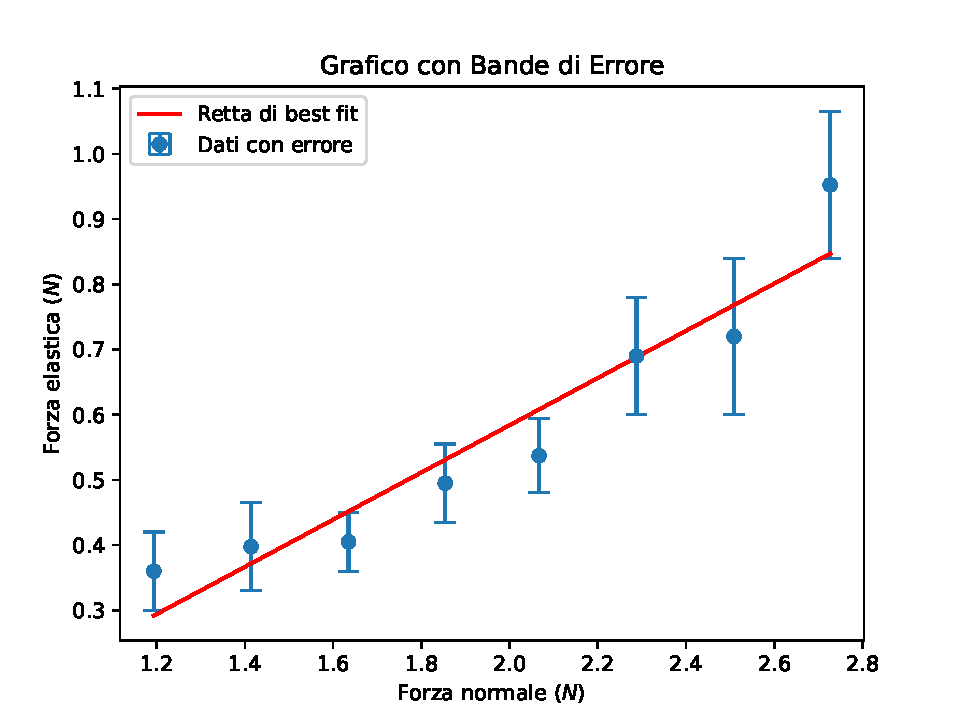
\includegraphics[width=0.99\textwidth]{grafico1.pdf}
  \caption{Il grafico mostra la forza elastica esercitata sul blocchetto in funzione della forza normale generata dalla superficie di contatto. \\
  Coefficiente angolare: $0.36\pm 0.14$ \\
  Intercetta: $-0.14\pm 0.29$ \\
  Questi parametri sono stati ottenuti utilizzando il metodo dei minimi quadrati (vedi Paragrafo 2.1).}
\end{figure}

\subsection{Seconda superficie}

\subsubsection{Prima massa}
\begin{table}[H]
\centering
\begin{tabular}{|c|c|}
\hline
\textbf{N°} & \textbf{$\Delta l_1$ ($cm$)}\\
\hline
$1$ & $20.50\pm 0.05$ \\
\hline
$2$ & $22.00\pm 0.05$ \\
\hline
$3$ & $21.50\pm 0.05$ \\
\hline
$4$ & $19.50\pm 0.05$ \\
\hline
$5$ & $21.00\pm 0.05$ \\
\hline
$6$ & $19.50\pm 0.05$ \\
\hline
$7$ & $20.50\pm 0.05$ \\
\hline
$8$ & $20.00\pm 0.05$ \\
\hline
$9$ & $20.00\pm 0.05$ \\
\hline
$10$ & $19.50\pm 0.05$ \\
\hline
$11$ & $20.00\pm 0.05$ \\
\hline
$12$ & $20.00\pm 0.05$ \\
\hline
$13$ & $20.00\pm 0.05$ \\
\hline
$14$ & $20.50\pm 0.05$ \\
\hline
$15$ & $20.50\pm 0.05$ \\
\hline
\end{tabular}
\caption{Allungamenti misurati per la prima massa.}
\label{tab:}
\end{table}
L'allungamento della molla è quindi:
\begin{equation}
    \Delta l_1=(20.75\pm 1.25)\ cm
\end{equation}
La forza elastica generata dalla molla è uguale a:
\begin{equation}
    F_{elastica_1} = (0.62\pm 0.04)\ N
\end{equation}
La forza normale agente sul blocchetto di legno è uguale a:
\begin{equation}
    F_{N_1} = (1.1938\pm 0.0001)\ N
\end{equation}

\subsubsection{Seconda massa}
\begin{table}[H]
\centering
\begin{tabular}{|c|c|}
\hline
\textbf{N°} & \textbf{$\Delta l_2$ ($cm$)}\\
\hline
$1$ & $26.50\pm 0.05$ \\
\hline
$2$ & $24.50\pm 0.05$ \\
\hline
$3$ & $24.00\pm 0.05$ \\
\hline
$4$ & $22.50\pm 0.05$ \\
\hline
$5$ & $23.50\pm 0.05$ \\
\hline
$6$ & $23.50\pm 0.05$ \\
\hline
$7$ & $22.50\pm 0.05$ \\
\hline
$8$ & $23.00\pm 0.05$ \\
\hline
$9$ & $23.50\pm 0.05$ \\
\hline
$10$ & $23.00\pm 0.05$ \\
\hline
$11$ & $23.00\pm 0.05$ \\
\hline
$12$ & $22.50\pm 0.05$ \\
\hline
$13$ & $22.50\pm 0.05$ \\
\hline
$14$ & $23.50\pm 0.05$ \\
\hline
$15$ & $22.00\pm 0.05$ \\
\hline
\end{tabular}
\caption{Allungamenti misurati per la seconda massa.}
\label{tab:}
\end{table}
L'allungamento della molla è quindi:
\begin{equation}
    \Delta l_2=(24.25\pm 2.25)\ cm
\end{equation}
La forza elastica generata dalla molla è uguale a:
\begin{equation}
    F_{elastica_7} = (0.73\pm 0.07)\ N
\end{equation}
La forza normale agente sul blocchetto di legno è uguale a:
\begin{equation}
    F_{N_2} = (1.4142\pm 0.0001)\ N
\end{equation}

\subsubsection{Terza massa}
\begin{table}[H]
\centering
\begin{tabular}{|c|c|}
\hline
\textbf{N°} & \textbf{$\Delta l_3$ ($cm$)}\\
\hline
$1$ & $28.00\pm 0.05$ \\
\hline
$2$ & $26.50\pm 0.05$ \\
\hline
$3$ & $27.50\pm 0.05$ \\
\hline
$4$ & $28.00\pm 0.05$ \\
\hline
$5$ & $26.50\pm 0.05$ \\
\hline
$6$ & $26.50\pm 0.05$ \\
\hline
$7$ & $27.50\pm 0.05$ \\
\hline
$8$ & $26.50\pm 0.05$ \\
\hline
$9$ & $26.50\pm 0.05$ \\
\hline
$10$ & $26.00\pm 0.05$ \\
\hline
$11$ & $26.50\pm 0.05$ \\
\hline
$12$ & $27.00\pm 0.05$ \\
\hline
$13$ & $27.00\pm 0.05$ \\
\hline
$14$ & $26.50\pm 0.05$ \\
\hline
$15$ & $26.50\pm 0.05$ \\
\hline
\end{tabular}
\caption{Allungamenti misurati per la terza massa.}
\label{tab:}
\end{table}
L'allungamento della molla è quindi:
\begin{equation}
    \Delta l_3=(27.00\pm 1.00)\ cm
\end{equation}
La forza elastica generata dalla molla è uguale a:
\begin{equation}
    F_{elastica_3} = (0.81\pm 0.03)\ N
\end{equation}
La forza normale agente sul blocchetto di legno è uguale a:
\begin{equation}
    F_{N_3} = (1.6350\pm 0.0001)\ N
\end{equation}

\subsubsection{Quarta massa}
\begin{table}[H]
\centering
\begin{tabular}{|c|c|}
\hline
\textbf{N°} & \textbf{$\Delta l_4$ ($cm$)}\\
\hline
$1$ & $30.00\pm 0.05$ \\
\hline
$2$ & $27.50\pm 0.05$ \\
\hline
$3$ & $27.00\pm 0.05$ \\
\hline
$4$ & $28.50\pm 0.05$ \\
\hline
$5$ & $26.00\pm 0.05$ \\
\hline
$6$ & $27.00\pm 0.05$ \\
\hline
$7$ & $28.00\pm 0.05$ \\
\hline
$8$ & $29.00\pm 0.05$ \\
\hline
$9$ & $28.00\pm 0.05$ \\
\hline
$10$ & $28.50\pm 0.05$ \\
\hline
$11$ & $31.00\pm 0.05$ \\
\hline
$12$ & $27.50\pm 0.05$ \\
\hline
$13$ & $29.50\pm 0.05$ \\
\hline
$14$ & $28.00\pm 0.05$ \\
\hline
$15$ & $29.50\pm 0.05$ \\
\hline
\end{tabular}
\caption{Allungamenti misurati per la quarta massa.}
\label{tab:}
\end{table}
L'allungamento della molla è quindi:
\begin{equation}
    \Delta l_4=(28.00\pm 2.50)\ cm
\end{equation}
La forza elastica generata dalla molla è uguale a:
\begin{equation}
    F_{elastica_4} = (0.86\pm 0.08)\ N
\end{equation}
La forza normale agente sul blocchetto di legno è uguale a:
\begin{equation}
    F_{N_4} = (1.8541\pm 0.0001)\ N
\end{equation}

\subsubsection{Quinta massa}
\begin{table}[H]
\centering
\begin{tabular}{|c|c|}
\hline
\textbf{N°} & \textbf{$\Delta l_5$ ($cm$)}\\
\hline
$1$ & $34.00\pm 0.05$ \\
\hline
$2$ & $32.50\pm 0.05$ \\
\hline
$3$ & $32.50\pm 0.05$ \\
\hline
$4$ & $31.50\pm 0.05$ \\
\hline
$5$ & $29.50\pm 0.05$ \\
\hline
$6$ & $33.50\pm 0.05$ \\
\hline
$7$ & $30.00\pm 0.05$ \\
\hline
$8$ & $30.00\pm 0.05$ \\
\hline
$9$ & $33.00\pm 0.05$ \\
\hline
$10$ & $34.50\pm 0.05$ \\
\hline
$11$ & $29.50\pm 0.05$ \\
\hline
$12$ & $30.50\pm 0.05$ \\
\hline
$13$ & $31.50\pm 0.05$ \\
\hline
$14$ & $32.50\pm 0.05$ \\
\hline
$15$ & $29.50\pm 0.05$ \\
\hline
\end{tabular}
\caption{Allungamenti misurati per la quinta massa.}
\label{tab:}
\end{table}
L'allungamento della molla è quindi:
\begin{equation}
    \Delta l_5=(32.00\pm 2.50)\ cm
\end{equation}
La forza elastica generata dalla molla è uguale a:
\begin{equation}
    F_{elastica_5} = (0.96\pm 0.08)\ N
\end{equation}
La forza normale agente sul blocchetto di legno è uguale a:
\begin{equation}
    F_{N_5} = (2.0669\pm 0.0001)\ N
\end{equation}

\subsubsection{Sesta massa}
\begin{table}[H]
\centering
\begin{tabular}{|c|c|}
\hline
\textbf{N°} & \textbf{$\Delta l_6$ ($cm$)}\\
\hline
$1$ & $36.00\pm 0.05$ \\
\hline
$2$ & $33.50\pm 0.05$ \\
\hline
$3$ & $35.50\pm 0.05$ \\
\hline
$4$ & $36.00\pm 0.05$ \\
\hline
$5$ & $36.00\pm 0.05$ \\
\hline
$6$ & $34.50\pm 0.05$ \\
\hline
$7$ & $34.00\pm 0.05$ \\
\hline
$8$ & $37.50\pm 0.05$ \\
\hline
$9$ & $33.00\pm 0.05$ \\
\hline
$10$ & $36.00\pm 0.05$ \\
\hline
$11$ & $36.00\pm 0.05$ \\
\hline
$12$ & $34.00\pm 0.05$ \\
\hline
$13$ & $36.00\pm 0.05$ \\
\hline
$14$ & $36.00\pm 0.05$ \\
\hline
$15$ & $34.50\pm 0.05$ \\
\hline
\end{tabular}
\caption{Allungamenti misurati per la sesta massa.}
\label{tab:}
\end{table}
L'allungamento della molla è quindi:
\begin{equation}
    \Delta l_6=(35.25\pm 2.25)\ cm
\end{equation}
La forza elastica generata dalla molla è uguale a:
\begin{equation}
    F_{elastica_6} = (1.06\pm 0.07)\ N
\end{equation}
La forza normale agente sul blocchetto di legno è uguale a:
\begin{equation}
    F_{N_6} = (2.2878\pm 0.0001)\ N
\end{equation}

\subsubsection{Settima massa}
\begin{table}[H]
\centering
\begin{tabular}{|c|c|}
\hline
\textbf{N°} & \textbf{$\Delta l_7$ ($cm$)}\\
\hline
$1$ & $39.00\pm 0.05$ \\
\hline
$2$ & $38.00\pm 0.05$ \\
\hline
$3$ & $36.00\pm 0.05$ \\
\hline
$4$ & $38.00\pm 0.05$ \\
\hline
$5$ & $38.00\pm 0.05$ \\
\hline
$6$ & $37.50\pm 0.05$ \\
\hline
$7$ & $38.50\pm 0.05$ \\
\hline
$8$ & $38.50\pm 0.05$ \\
\hline
$9$ & $39.90\pm 0.05$ \\
\hline
$10$ & $41.00\pm 0.05$ \\
\hline
$11$ & $37.00\pm 0.05$ \\
\hline
$12$ & $37.00\pm 0.05$ \\
\hline
$13$ & $38.50\pm 0.05$ \\
\hline
$14$ & $36.00\pm 0.05$ \\
\hline
$15$ & $38.00\pm 0.05$ \\
\hline
\end{tabular}
\caption{Allungamenti misurati per la settima massa.}
\label{tab:}
\end{table}
L'allungamento della molla è quindi:
\begin{equation}
    \Delta l_7=(38.50\pm 2.50)\ cm
\end{equation}
La forza elastica generata dalla molla è uguale a:
\begin{equation}
    F_{elastica_7} = (1.16\pm 0.08)\ N
\end{equation}
La forza normale agente sul blocchetto di legno è uguale a:
\begin{equation}
    F_{N_7} = (2.5088\pm 0.0001)\ N
\end{equation}

\subsubsection{Ottava massa}
\begin{table}[H]
\centering
\begin{tabular}{|c|c|}
\hline
\textbf{N°} & \textbf{$\Delta l_8$ ($cm$)}\\
\hline
$1$ & $42.00\pm 0.05$ \\
\hline
$2$ & $41.00\pm 0.05$ \\
\hline
$3$ & $47.00\pm 0.05$ \\
\hline
$4$ & $44.00\pm 0.05$ \\
\hline
$5$ & $43.50\pm 0.05$ \\
\hline
$6$ & $38.00\pm 0.05$ \\
\hline
$7$ & $43.50\pm 0.05$ \\
\hline
$8$ & $43.50\pm 0.05$ \\
\hline
$9$ & $41.00\pm 0.05$ \\
\hline
$10$ & $40.50\pm 0.05$ \\
\hline
$11$ & $42.50\pm 0.05$ \\
\hline
$12$ & $41.50\pm 0.05$ \\
\hline
$13$ & $38.00\pm 0.05$ \\
\hline
$14$ & $43.00\pm 0.05$ \\
\hline
$15$ & $40.50\pm 0.05$ \\
\hline
\end{tabular}
\caption{Allungamenti misurati per l'ottava massa.}
\label{tab:}
\end{table}
L'allungamento della molla è quindi:
\begin{equation}
    \Delta l_8=(42.50\pm 4.50)\ cm
\end{equation}
La forza elastica generata dalla molla è uguale a:
\begin{equation}
    F_{elastica_8} = (1.28\pm 0.14)\ N
\end{equation}
La forza normale agente sul blocchetto di legno è uguale a:
\begin{equation}
    F_{N_8} = (2.7266\pm 0.0001)\ N
\end{equation}

\subsubsection{Secondo grafico}
\begin{figure}[H]
  \centering
  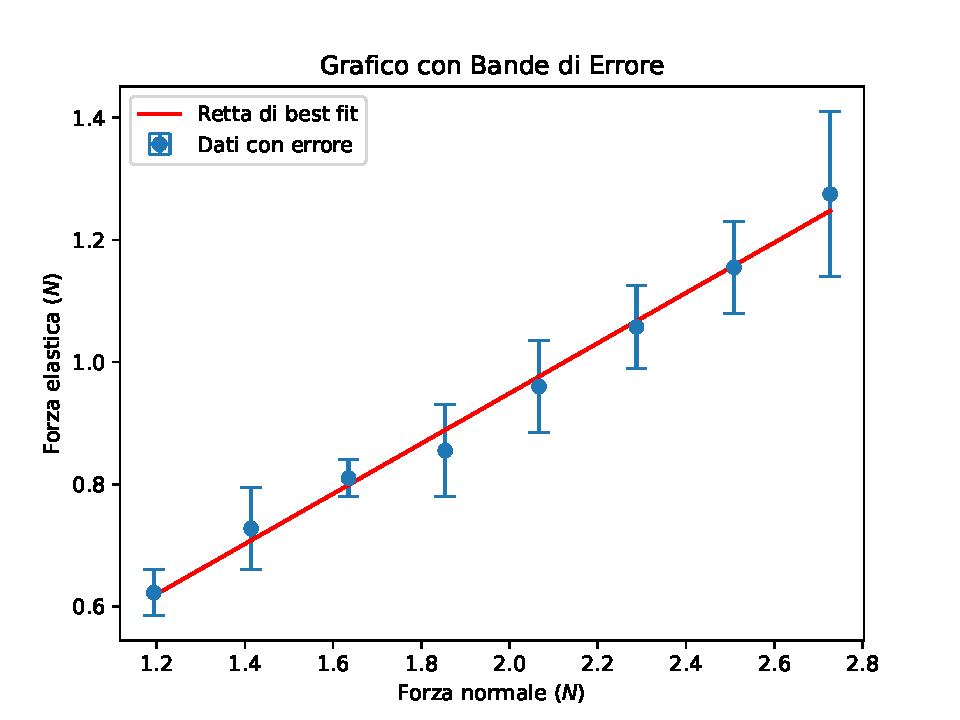
\includegraphics[width=0.99\textwidth]{grafico2.pdf}
  \caption{Il grafico mostra la forza elastica esercitata sul blocchetto in funzione della forza normale generata dalla superficie di contatto. \\
  Coefficiente angolare: $0.41\pm 0.05$ \\
  Intercetta: $0.13\pm 0.10$ \\
  Questi parametri sono stati ottenuti utilizzando il metodo dei minimi quadrati (vedi Paragrafo 2.1).}
\end{figure}

\section{Conclusioni}
Dalla Legge (1) notiamo che la forza elastica in funzione della forza normale segue un andamento lineare e il suo coefficiente angolare è proprio il coefficiente di attrito statico $\mu_s$. I coefficienti angolari dei grafici (3) e (4) rappresentano quindi il coefficiente di attrito statico.
\begin{itemize}
    \item $\mu_{s_1} = (0.36\pm 0.14)$
    \item $\mu_{s_2} = (0.41\pm 0.05)$
\end{itemize}
I due coefficienti di attrito statico, considerando i soli valori assoluti, sono molto simili. L'attrito non dipende dalla dimensione della superficie di contatto ma solo dalle sue caratteristiche chimico-fisiche. I risultati ottenuti sono quindi validi e rispecchiano i valori attesi.

\end{document}